\section{HTTPS}

\begin{defi}{Web-Security}
    Webanwendungen sind mehr als nur öffentliche Webseiten im Browser.
    Jede Client-Server-Anwendung, die auf Webtechnologien basiert, ist eine Webanwendung.

    Durch neue Entwicklungen wird die Anwendungslogik von Server zum Client verlagert\footnote{in JavaScript z. B. durch AJAX, Singe-Page-Applications, Web- und Microservices, REST etc.}.

    Es stehen neue Virtualisierungstechnologien wie z. B. Docker zur Verfügung.
\end{defi}

\begin{defi}{IT-Sicherheit}
    \emph{IT-Sicherheit} ist definiert als Schutz der \emph{Infrastrukturschichten}\footnote{Netzzugangs-, Internet- und Transportschicht in TCP/IP} z. B. durch:
    \begin{itemize}
        \item Firewall und Reverse Proxy
        \item Intrusion Detection (IDS) bzw. Prevention System (IPS)
    \end{itemize}

    Ein überwiegender Teil aller Angriffe findet jedoch auf der Anwendungsschicht mittels HTTP-Protokoll statt.
\end{defi}

\begin{defi}{Strukturelle Sicherheitsprobleme HTTP}
    \begin{itemize}
        \item HTTP ist unverschlüsselt und ohne Integritätsschutz
        \item HTTP ist zustandslos. Nötige Daten müssen in weiteren Requests mitgesendet werden, z. B. durch Sessions.
        \item Kommunikation durch nicht typisierte URL-Parameter
        \item Unsichere eingebaute Authentifizierungsverfahren
    \end{itemize}
\end{defi}

\begin{defi}{Schutzziele}
    Primäre Schutzziele (\emph{CIA Triad}):
    \begin{itemize}
        \item \emph{Vertraulichkeit (Confidentiality)}:
              \begin{itemize}
                  \item Übertragene Daten sind nur befugten Personen zugänglich.
                  \item Ansatz: symmetrische und asymmetrische Verschlüsselung, HTTPS
              \end{itemize}
        \item \emph{Integrität (Integrity)}:
              \begin{itemize}
                  \item Übertragene Daten sind nachweislich vollständig und unverändert.
                  \item Ansatz: Message Authentication Code (MAC)
              \end{itemize}
        \item \emph{Verfügbarkeit (Availability)}:
              \begin{itemize}
                  \item Datenzugriff steht (befugten Personen) bei Bedarf zur Verfügung.
                  \item Angriff: (Distributed) Denial of Service z. B. \texttt{SYN-Flood} beim TCP-Verbindungsaufbau
              \end{itemize}
    \end{itemize}

    Sekundäre Schutzziele:
    \begin{itemize}
        \item Authentizität (Authenticity)
        \item Zurechenbarkeit (Accountability)
        \item Verbindlichkeit (Non-Repudiation)
    \end{itemize}
\end{defi}

\begin{bonus}{Kryptographie}
    \emph{Symmetrische Verschlüsselung}:
    \begin{itemize}
        \item Gleicher Schlüssel für Ver- und Entschlüsselung
        \item Jede Verbindung benötigt einen eigenen Schlüssel
        \item Nachteile:
              \begin{itemize}
                  \item Geheimhaltung und sicherer Austausch des Schlüssels nötig.
                  \item Schuld an kompromittierten Schlüsseln nicht eindeutig.
              \end{itemize}
        \item Beispiele:
              \begin{itemize}
                  \item One-Time-Pad (1882)
                  \item DES (1975)
                  \item Blowfish (1993)
                  \item Twofish (1998)
                  \item Serpent (1998)
                  \item AES (1998)
              \end{itemize}
    \end{itemize}

    \emph{Asymmetrische Verschlüsselung}:
    \begin{itemize}
        \item Verschiedene Schlüssel für Ver- und Entschlüsselung
        \item Jeder Client hat z. B. einen privaten und einen öffentlichen Schlüssel:
              \begin{itemize}
                  \item Beim \emph{Versenden} wird der öffentliche Schlüssel des Empfängers zum Verschlüsseln verwendet.
                  \item Beim \emph{Empfangen} wird der eigene private Schlüssel zum Entschlüsseln genutzt.
                  \item Zum Authentifizieren verschlüsselt man eine öffentliche Nachricht\footnote{z. B. seine MAC-Adresse} mit seinem privaten Schlüssel.
                        Wenn der erwartete Inhalt beim Entschlüsseln mit dem öffentlichen Schlüssel des Geräts erhalten wird, ist der Client authentifiziert\footnote{Wenn Dritte Zugriff zu dem privaten Schlüssel erhalten, können sie sich als das betroffene Gerät ausgeben.}.
              \end{itemize}
        \item Nachteile:
              \begin{itemize}
                  \item langsam
              \end{itemize}
        \item Beispiele:
              \begin{itemize}
                  \item RSA
                  \item Diskreter Logarithmus (DL)
                  \item Elliptische Kurven (EC)
              \end{itemize}
    \end{itemize}
\end{bonus}

\begin{bonus}{Kryptographische Hashfunktion}
    Eigenschaften:
    \begin{itemize}
        \item \emph{Kompression}: bildet beliebig lange Bitfolgen auf eine Bitfolge fester Länge ab
        \item \emph{Effizienz}: Hashwert für gegebene Bitfolge \enquote{leicht} berechenbar
        \item \emph{Einweg}: \enquote{schwer} für einen gegeben Hashwert eine Bitfolge zu finden, die diesen Hashwert besitzt
    \end{itemize}

    Anwendungsfälle:
    \begin{itemize}
        \item Prüfsummen und Fingerprints zum schnellen Vergleichen großer Daten
        \item Integritätsprüfung von Nachrichten
        \item Sichere Speicherung von Passwörtern und digitalen Signaturen
        \item Pseudo-Zufallsgeneratoren
    \end{itemize}
\end{bonus}

\begin{defi}{HTTPS}
    HTTP ist unverschlüsselt.
    Jeder Man-in-the-Middle kann daher die Kommunikation mitschneiden und verändern.

    Um sicherzugehen, dass Inhalte vom Server stammen und unverändert ausgeliefert wurden, muss \emph{HTTPS} genutzt werden.

    \emph{HTTPS} verschlüsselt alle Inhalte, außer IP-Adressen und Ports.
\end{defi}

\begin{bonus}{SSL}
    \emph{Secure Socket Layer (SSL)} stellt mit Hilfe digitaler Zertifikate sicher, dass die übertragenen Inhalte durch symmetrische Algorithmen verschlüsselt werden.

    Beim Verbindungsaufbau wird sich auf einen symmetrischen Schlüssel geeinigt, mit dem die Daten verschlüsselt werden.

    Der Verbindungsaufbau erfolgt jedoch mit asymmetrischer Verbindung.
\end{bonus}

\begin{bonus}{TLS}
    \emph{Transport Layer Security (TLS)} ist eine Weiterentwicklung von SSL und wird heutzutage fast ausschließlich genutzt.
\end{bonus}

\begin{defi}{TLS Handshake Protocol}
    Das \emph{TLS Handshake Protocol} baut auf dem TLS Record Protocol auf und erfüllt die folgenden Funktionen, noch bevor die ersten Bits des Anwendungsdatenstromes ausgetauscht wurden:
    \begin{itemize}
        \item Aushandeln zu benutzender kryptografischer Algorithmen und Schlüssel. TLS unterstützt auch eine unverschlüsselte Übertragung.
        \item Identifikation und Authentifizierung der Kommunikationspartner auf Basis asymmetrischer Verschlüsselungsverfahren und Public-Key-Kryptografie.\footnote{Dieser Schritt ist optional eine Zwei-Wege-Authentifizierung (in diesem Fall wird manchmal von mutual TLS gesprochen), für gewöhnlich authentifiziert sich aber nur der Server gegenüber dem Client.}
    \end{itemize}

    Insgesamt besteht der TLS Handshake aus vier Phasen:
    \begin{enumerate}
        \item Der Client schickt zum Server ein \texttt{ClientHello}, und der Server antwortet dem Client mit einem \texttt{ServerHello}. Die Parameter der Nachrichten sind:
              \begin{itemize}
                  \item die Version (die höchste vom Client unterstützte TLS-Protokoll-Version)
                  \item eine 32 Byte lange Zufallsinformation
                  \item eine Session-ID
              \end{itemize}
        \item Der Server identifiziert sich gegenüber dem Client.
              \begin{itemize}
                  \item Hierzu wird per Certificate ein \emph{X.509-Zertifikat} an den Client geschickt, gefolgt von einem \texttt{CertificateVerify} (in einigen TLS Versionen).
                  \item Die \texttt{CertificateVerify} Nachricht enthält eine Unterschrift von zuvor ausgetauschten Nachrichten.
                  \item Der Client prüft das Zertifikat und die Unterschrift. Bei Misserfolg bricht der Client die Verbindung ab.
                  \item Außerdem kann der Server optional per \texttt{CertificateRequest} ein Zertifikat zur Client-Authentifizierung anfordern.
              \end{itemize}
        \item Das zuvor erhaltene Server-Zertifikat enthält den öffentlichen Schlüssel des Servers. Es wird ein Diffie-Hellman-Schlüsselaustausch durchgeführt, um ein gemeinsames \emph{pre-master-secret} zu generieren.
        \item Diese Phase schließt den Handshake ab. Aus dem vorhandenen pre-master-secret kann das \emph{master secret} abgeleitet werden, das einen einmaligen \emph{Sitzungsschlüssel (Session Key)} darstellt.
              \begin{itemize}
                  \item Aus dem master secret werden wiederum \emph{Schlüssel} abgeleitet, die zum Ver- und Entschlüsseln der Daten sowie für die Integritätsprüfung verwendet werden.
                  \item Die Nachrichten, die die Kommunikationspartner sich nun gegenseitig zusenden, werden nur noch verschlüsselt übertragen.
              \end{itemize}
    \end{enumerate}
\end{defi}

\begin{defi}{TLS Record Protocol}
    Das \emph{TLS Record Protocol} dient zur Absicherung der Verbindung.

    Es setzt direkt auf der Transportschicht auf und bietet zwei verschiedene Dienste, die einzeln oder gemeinsam genutzt werden können:
    \begin{itemize}
        \item Ende-zu-Ende-Verschlüsselung mittels symmetrischer Algorithmen. Der verwendete Schlüssel wird dabei im Voraus über ein weiteres Protokoll (zum Beispiel das TLS Handshake Protocol) ausgehandelt und kann nur einmal für die jeweilige Verbindung verwendet werden.
        \item Sicherung der Nachrichten-Integrität und Authentizität durch einen Message Authentication Code (MAC).
    \end{itemize}
\end{defi}

\begin{bonus}{X.509 Zertifikat}
    \emph{X.509} ist ein Standard für eine Public-Key-Infrastruktur zum Erstellen digitaler Zertifikate.

    In der elektronischen Kommunikation finden X.509-Zertifikate Anwendung bei den TLS-Versionen diverser Übertragungsprotokolle, wie z. B. beim Abruf von Web-Seiten mit HTTPS oder zum Unterschreiben und Verschlüsseln von E-Mails nach dem S/MIME-Standard.

    Struktur eines X.509-v3-Zertifikats:
    \begin{itemize}
        \item Zertifikat
              \begin{itemize}
                  \item Version
                  \item Seriennummer
                  \item Algorithmen-ID
                  \item Aussteller
                  \item Gültigkeit
                        \begin{itemize}
                            \item von
                            \item bis
                        \end{itemize}
                  \item Zertifikatinhaber
                  \item Zertifikatinhaber-Schlüsselinformationen
                        \begin{itemize}
                            \item Public-Key-Algorithmus
                            \item Public Key des Zertifikatinhabers
                        \end{itemize}
                  \item Eindeutige ID des Ausstellers (optional)
                  \item Eindeutige ID des Inhabers (optional)
                  \item Erweiterungen (optional)
              \end{itemize}
        \item Zertifikat-Signaturalgorithmus
        \item Zertifikat-Signatur
    \end{itemize}
\end{bonus}

\begin{defi}{HTTPS-Zertifikat}
    Ein \emph{HTTPS-Zertifikat} besteht aus:
    \begin{itemize}
        \item Versionsnummer
        \item Seriennummer
        \item Signaturalgorithmus
        \item Aussteller
        \item Gültigkeit
        \item Subjekt
        \item SubjectPublicKeyInfo
        \item Signatur
    \end{itemize}
\end{defi}

\begin{defi}{Signatur}
    Eine \emph{digitale Signatur} ist ein asymmetrisches Kryptosystem, bei dem ein Sender mit Hilfe eines geheimen Signaturschlüssels (dem Private Key) zu einer digitalen Nachricht (d. h. zu beliebigen Daten) einen Wert berechnet, der ebenfalls digitale Signatur genannt wird.
    Dieser Wert ermöglicht es jedem, mit Hilfe des öffentlichen Verifikationsschlüssels (dem Public Key) die nichtabstreitbare Urheberschaft und Integrität der Nachricht zu prüfen.

    Um eine mit einem Signaturschlüssel erstellte Signatur einer Person zuordnen zu können, muss der zugehörige Verifikationsschlüssel dieser Person zweifelsfrei zugeordnet sein.

    Bei einer digitalen Signatur wird der private Schlüssel in der Regel nicht direkt auf die Nachricht angewendet, sondern auf deren Hash-Wert, der mittels einer Hashfunktion (wie z. B. SHA-1) aus der Nachricht berechnet wird.

    Um Angriffe zu verhindern, muss diese Hashfunktion kollisionsresistent sein, d. h., es muss praktisch unmöglich sein, zwei unterschiedliche Nachrichten zu finden, deren Hash-Wert identisch ist.
\end{defi}

\begin{bonus}{CAs}
    Die \emph{Certificate Authorities (CAs)} stellen u. a. für Webseitenbetreibende Zertifikate aus und signieren diese.

    Vertraut ein Client der CA, vertraut er auch dem ausgestellten Zertifikat.

    Browser und Betriebssysteme kommen mit einer Reihe voreingestellten \emph{Trusted Root CAs}.
    Diese können selbstsignierte Zertifikate ausstellen, müssen jedoch längere Verfahren durchlaufen bis Browserhersteller oder Betriebssysteme die CA aufnehmen.
    Browser speichern Trusted Root CAs.

    z. B. von \href{https://www.fh-aachen.de}{https://www.fh-aachen.de}: \enquote{Systems Enterprise Services GmbH}

    \emph{Trusted CAs} können beliebige Zertifikate ausstellen.
\end{bonus}

\begin{bonus}{Probleme CAs}
    Es existiert eine \emph{Common CA Database (CCADB)}, in der \emph{Root Zertifikate} gespeichert sind.

    Mitglieder sind z. B.:
    \begin{itemize}
        \item Mozilla
        \item Microsoft
        \item Google
    \end{itemize}

    Ein einziger kompromittierter \emph{CA} gefährdet das gesamte Web.
    In zahlreichen Vorfällen wurden in der Vergangenheit mehrere \emph{private Schlüssel} durch Angriffe veröffentlicht.

    Der Einsatz von Zertifikaten erfordert Wissen um die Prozesse zur Erstellung von Zertifikaten.
    Zusätzlich müssen Zertifikate gepflegt werden und können auslaufen.
\end{bonus}

\begin{bonus}{PKI}
    Die \emph{Public Key Infrastructure (PKI)} besteht aus:
    \begin{itemize}
        \item \emph{Registrierungsstelle}:
              \begin{itemize}
                  \item Organisationen, bei der Personen, Maschinen oder auch untergeordnete Zertifizierungsstellen Zertifikate beantragen können
                  \item prüft Richtigkeit der Daten im gewünschten Zertifikat und genehmigt Zertifikatsantrag, der dann durch eine Zertifizierungsstelle signiert wird
              \end{itemize}
        \item \emph{Zertifizierungsstelle}:
              \begin{itemize}
                  \item vertrauenswürdige Organisation, die Signatur von Zertifikatsanträgen gemäß bekannter Regeln übernimmt
              \end{itemize}
        \item \emph{Verzeichnisdienst}:
              \begin{itemize}
                  \item durchsuchbares Verzeichnis, das ausgestellte Zertifikate enthält
              \end{itemize}
        \item \emph{Validierungsdienst}:
              \begin{itemize}
                  \item Dienst, der Überprüfung von Zertifikaten in Echtzeit ermöglicht
              \end{itemize}
    \end{itemize}
\end{bonus}

\begin{bonus}{POODLE-Attacke}
    \emph{Padding Oracle On Downgraded Legacy Encryption}-Attacken reduzieren Verbindungen auf niedrigere SSL-Versionen.
\end{bonus}

\begin{defi}{HSTS}
    \emph{Strict Transport Security (HSTS)} teilt einem Browser mit, dass eine Seite nur über HTTPS und den angegeben \emph{Cipher Suites} erreichbar ist.

    Sobald man einmal mit einer Webseite verbunden ist, merkt sich der Browser die Verbindungseigenschaften.

    Dadurch werden \emph{POODLE}-Attacken verhindert.
\end{defi}

\begin{defi}{HPKP}
    \emph{HTTP Public Key Pinning (HPKP)} setzt den Browser auf einen öffentlichen Schlüssel fest.

    Danach kann niemand versuchen die Identität des Servers mit einem gefälschten Zertifikat anzunehmen.

    Dieses System wurde im Jahr 2020 deaktiviert.
\end{defi}

\begin{bonus}{TLS-Terminierung bei Reverse Proxy}
    \begin{center}
        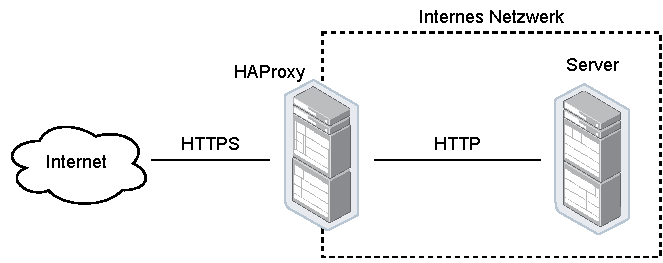
\includegraphics[width=0.75\textwidth]{includes/figures/bonus_tls_reverse_proxy.pdf}
    \end{center}
\end{bonus}